\section{Servo motor}
The purpose of the servo motor is control the "flipper", which separates the blocks. \\


A servo motor consist of an DC motor, potentiometer and a control circuit.  As the motor rotates, the resistance of the potentiometer changes,  which the the control circuit  uses and  regulate its movement and the direction based on it.   When the motor shaft is at the desired position the power supplied to the motor will be used stop the motor, such that it doesn't move away from the desired position. \\

The desired position is sent through the sense wire, (often the white wire). The position itself is defined as the duty cycle of the PWM signal that it is provided with, as seen on \ref{fig:Servo_position}. 
 
\begin{figure}[H]
\centering
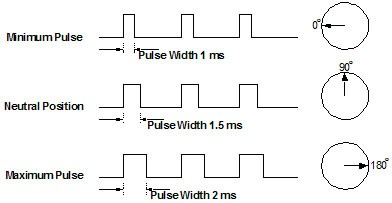
\includegraphics[scale=0.6]{images/servocontrol.jpg}
\label{fig:Servo_position}
%http://www.societyofrobots.com/actuators_servos.shtml
\end{figure}

\subsection{Interaction with Servo motor}
The control of the servo motor, is done using the FPGA with the entity named pwm. 

\begin{figure}[htb]
\centering
\begin{tikzpicture}[font=\sffamily,>=triangle 45]
  \node [shape=circuit] (item) at (0,0) {pwm};
  \draw [<-] (item.ina) node [anchor=west,labels] {} -- +(-1,0) node [anchor=east] {CLK};
  \draw [->] (item.outa) node [anchor=east,labels] {} -- +(1,0) node [anchor=west] {PWM\_motor};
  \draw [<-] (item.inb) node [anchor=west,labels] {} -- +(-1,0) node [anchor=east] {direc};
\end{tikzpicture}
\caption{Entity of pwm}
\end{figure}

\texttt{PWM\_motor} is connected to servo motor, and provides the PWM signal that sets the position of it. 
\texttt{direc} is an input signal, which tells the entity which direction the servo motor has to move to, and thereby deciding the duty cycle of the PWM signal. \texttt{CLK} is the clock frequency of the FPGA. \\

The component has only one process, that generates 3 different pwm signals based on the value of \texttt{direc}. If \texttt{direc} is "11" it moves to the right, if it is "00" it moves to the left, and if it has  other value it will stay neutral . \\


The period of the pwm signal of \texttt{PWM\_motor} is set to  20 ms, which the servo motors requires. 
For each  \texttt{rising\_edge} of the \texttt{CLK} a variable named \texttt{count} is incremented.  To make the motor move to left, will \texttt{PWM\_motor} stay zero until \texttt{count} is below 950000 and when it above 950000  and below 1000000 it will stay high, as 50000 \texttt{rising\_edge} equate to 1 ms. When count has reached 1000000 will it be reset again. \\




